\clearpage
\section{Tiny Garble}

\begin{refsection}

\begin{tcolorbox}	
\begin{tabular}{p{2.75cm} p{0.2cm} p{10.5cm}} 	
\textbf{Students Name}      &:& Goncalo Vitor (15/06/2018 - )\\
\textbf{Goal}               &:& Implementation of secure multy-party computation based on the Tiny Garble framework.\\
\textbf{Directory}          &:& \\
\end{tabular}
\end{tcolorbox}



This subsection will cover the installation and usage of TinyGarble, a GC framework that allows two parties to safely compute any function with their private inputs through Yao's Garbled Circuit Potocol. It accepts HDL and C/C++ as user inputs, although HDL will be the primary focus.

\subsection{Installation}

Since TinyGarble and most of the tools mentioned below have been mostly tested on Linux, it will be assumed that the user is running Linux on a virtual machine (VM), or directly from a partition. To do the former one can use Oracle's VirtualBox, which can be downloaded at \url{https://www.virtualbox.org/wiki/Downloads}. A copy of Linux is also needed, for this section Ubuntu 18.04 was used, found at \url{https://www.ubuntu.com/download/desktop}.

After installing and opening VirtualBox, select 'New', a Window should pop up asking for a name for the new VM, it doesn't matter, and for type and version, which should be Linux and Ubuntu respectively. The next step is choosing the amount of RAM that is going to be dedicated to the VM,  it depends on the system, but anything between 2048 and 4096 MB should be fine, 1024 MB or lower if the host PC has small amount of memory. Next create a virtual hard disk of VDI type, and choose dynamic or fixed size disk, it comes down to user preference. For the size of the disk, 10GB was enough to install and use TinyGarble properly, but slightly more is advisable.
After creating the virtual machine, it should ask for a start-up disk when launching it for the first time, select the Linux ISO file that was downloaded before. After that the installation of linux is pretty straight forward.

For TinyGarble to work, some dependencies have to be installed first, on Ubuntu it can be done with the following lines:

\begin{lstlisting}[caption={Installation of TinyGarble's dependencies}, language=bash, captionpos=b]
$ sudo apt install git
$ sudo apt install build-essential
$ sudo apt install libssl1.0-dev
$ sudo apt install libboost-all-dev
$ sudo apt install cmake
\end{lstlisting}

After this step i'ts necessary to clone TinyGarble's repository, at \url{https://github.com/esonghori/TinyGarble}, and build it.

\begin{lstlisting}[caption={Configuration and compilation of TinyGarble}, language=bash, captionpos=b]
$ git clone https://github.com/esonghori/TinyGarble.git
$ cd TinyGarble/
$ ./configure
$ cd bin/
$ make
\end{lstlisting}

To be able to use TinyGarble, a RTL Synthesis tool is also needed, to translate Verilog files into Netlist ones. In the example showed later, Yosys-abc is used. Which can be installed on Ubuntu 15.04 or higher with:

\begin{lstlisting}[caption={Installation of Yosys-abc for Ubuntu 15.04>}, language=bash, captionpos=b]
$ sudo apt-get install yosys
\end{lstlisting}

If on Ubuntu 14.04 or lower, a repository needs to be added first:

\begin{lstlisting}[caption={Installation of Yosys-abc for Ubuntu 14.04<}, language=bash, captionpos=b]
$ sudo add-apt-repository ppa:saltmakrell/ppa
$ sudo apt update
$ sudo apt install yosys
\end{lstlisting}

\newpage

\subsection{Usage}

\begin{figure}[H]
	\centering
	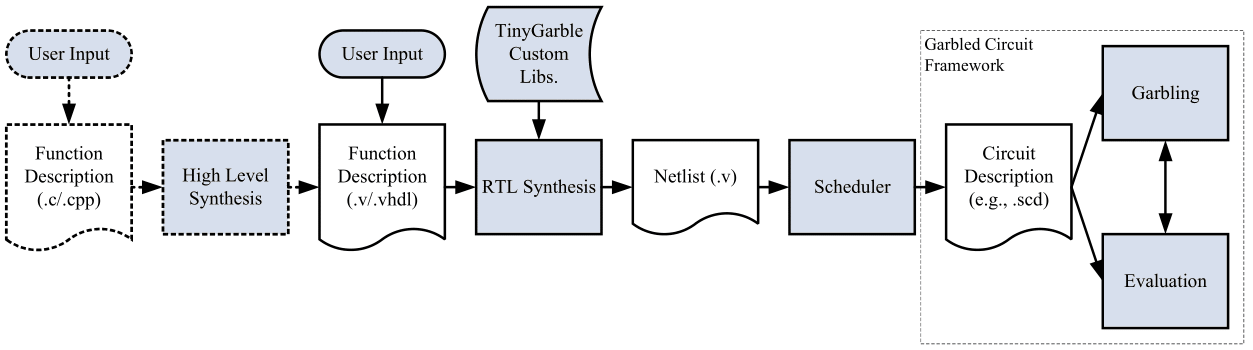
\includegraphics[width=1\textwidth, height=3cm]{./sdf/secure_multiparty_computation/figures/tiny_garble_flow.png}
    \caption{TinyGarble Global Flow\cite{Songhori}}\label{fig:tinygarble_flow}
\end{figure}

Following TinyGarble's global flow showed on the image above, it's possible to see that a C/C++ or Hardware Design Language (HDL) input is necessary. The former is slightly worse in terms of performance, since it needs an extra step of synthesis, with the help of a High Level Synthesis (HLS) tool, like Spart or Xilinx Vivado for C, to compile the C/C++ file into HDL, causing the end SCD file to have more logical gates than when using HDL input directly. This section mostly covers Verilog, since it's the most direct input, if VHDL input is needed, check \ref{ssec:usingVHDL}.

When writting the input file, some attention to the circuit's ports is needed, since TinyGarble's V2SCD (Netlist Verilog to SCD converter) accepts netlist files with a special format.
Below are the ports that can be used and what they represent.

\begin{itemize}
\item clk: clock cycle
\item rst: active high reset
\item g\_init: garbler's initial values (read at the first clock)
\item e\_init: evaluator's initial values (read at the first clock)
\item g\_input: garbler's input (read at every clock)
\item e\_input: evaluator's input (read at every clock)
\item o: output
\end{itemize}

Below it's an example of an and\_gate written in verilog with the format above.

\begin{lstlisting}[caption={and\_gate.v}, language=Verilog, captionpos=b]
module and_gate (input g_input, e_input, output o);
	assign o = g_input & e_input;
endmodule
\end{lstlisting}

Using TinyGarble's custom library, asic\_cell\_yosys\_extended.lib", located at TinyGarble/ciruit\_synthesis/lib/, and assuming that the Verilog file is located at a folder named "circuits", the compilation can be done with the following instructions:

\begin{lstlisting}[caption={Yosys instructions to compile the HDL file to a Netlist file}, language=bash, captionpos=b]
$ ./yosys
yosys> read_verilog circuits/and_gate.v
yosys> hierarchy -check -top and_gate
yosys> proc; opt; memory; opt; fsm; opt; techmap; opt;
yosys> abc -liberty TinyGarble/circuit_synthesis/lib/
asic_cell_extended.lib
yosys> clean
yosys> write_verilog circuits/and_gate_netlist.v
yosys> exit					
\end{lstlisting}

Following these, the Netlist file below should be generated.

\begin{lstlisting}[caption={and\_gate\_netlist.v}, language=Verilog, captionpos=b]
(* top =  1  *)
(* src = "and.v:1" *)
module and_gate( g_input,  e_input, o);
  (* src = "and.v:2" *)
  input g_input;
  (* src = "and.v:2" *)
  input e_input;
  (* src = "and.v:3" *)
  output o;
  AND _0_ (
    .A(e_input),
    .B(g_input),
    .Z(o)
  );
endmodule
\end{lstlisting}

For some unkown reason, the output file has some noticeably weird lines, starting with "(*", that will cause Segmentation Fault error in the next step if not removed.
After removing those lines, the Netlist file can be converted into a SCD file with the instruction below:

\begin{lstlisting}[caption={Installation of Yosys-abc}, language=bash, captionpos=b]
$ ./TinyGarble/bin/scd/V2SCD_Main -i circuits/and_gate_netlist.v
-o circuits/and_gate.scd		
\end{lstlisting}

Before executing the SCD file, it can be tested with TinyGarble's SCD\_Evaluator\_Main located at TinyGarble/bin/scd, with the code below:

\begin{lstlisting}[caption={Testing a SCD file}, language=bash, captionpos=b]
$ ./TinyGarble/bin/scd/SCD_Evaluator_Main -i circuits/and_gate --g_input 1 --e_input 0
\end{lstlisting}

\newpage

The SCD file can now be executed by both parties, "Alice" and "Bob", as shown on the upper terminal and lower terminal of the following images, respectively.
For this examples the SCD file was located at TinyGarble/bin/garbled\_circuits, same directory where the instructions were executed.

\begin{figure}[H]
	\centering
	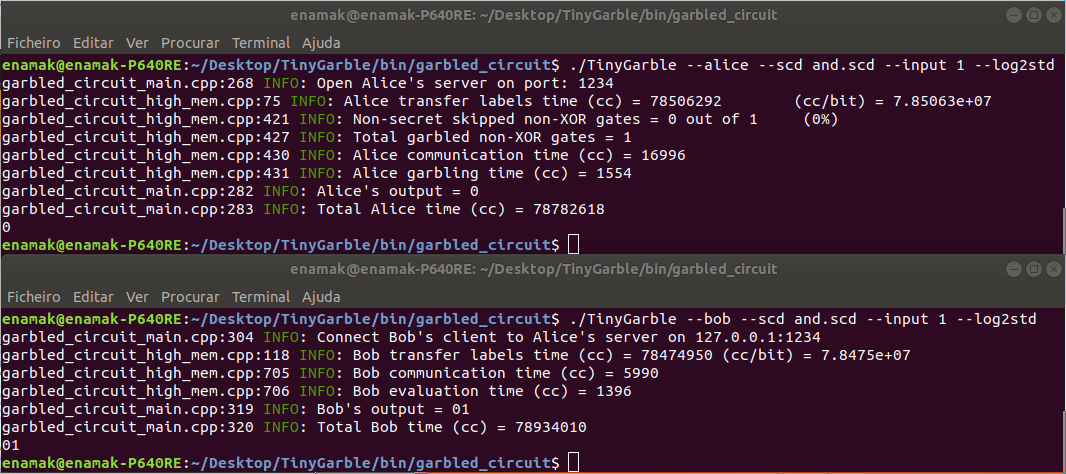
\includegraphics[width=1\textwidth, height=7cm]{./sdf/secure_multiparty_computation/figures/tinygarble_and_a.png}
    \caption{"And" function executed by Alice and Bob, with inputs 1 and 1, respectively}\label{fig:tinygarble_and_a}
\end{figure}

\begin{figure}[H]
	\centering
	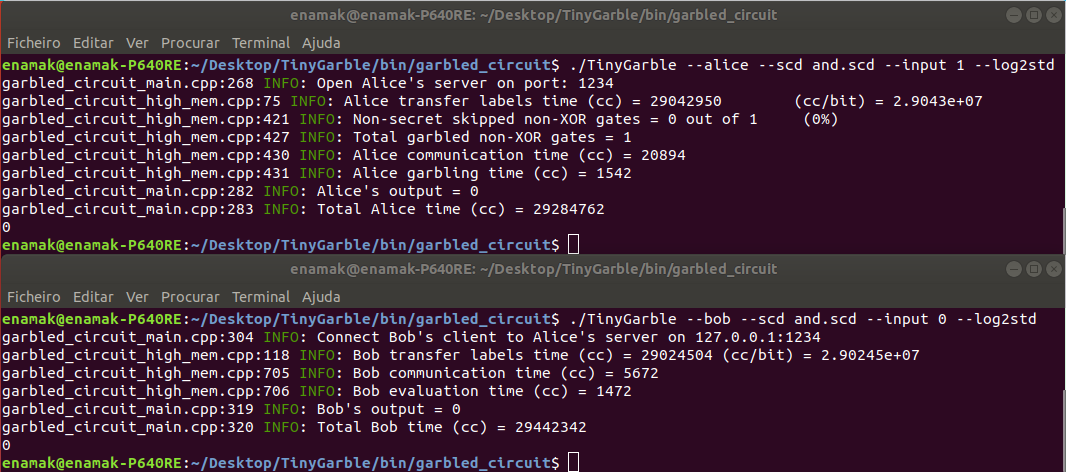
\includegraphics[width=1\textwidth, height=7cm]{./sdf/secure_multiparty_computation/figures/tinygarble_and_b.png}
    \caption{"And" function executed by Alice and Bob, with inputs 1 and 0, respectively}\label{fig:tinygarble_and_b}
\end{figure}

The input is written in hexadecimal, and the log2std option is to show information of the computation on the terminal instead of creating a log file.

\begin{figure}[H]
	\centering
	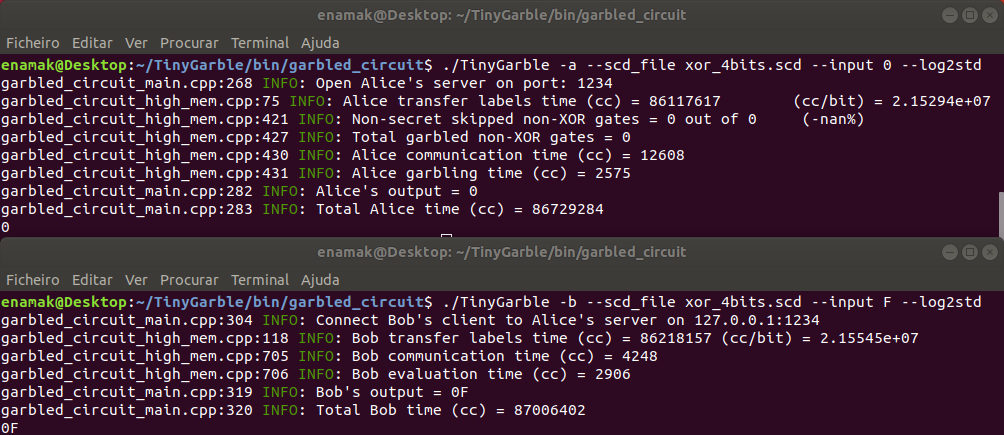
\includegraphics[width=1\textwidth, height=7cm]{./sdf/secure_multiparty_computation/figures/tinygarble_xor_4bits_b.png}
    \caption{"Xor" function with 4 bits, executed by Alice and Bob, with inputs 0 and F, respectively}\label{fig:tinygarble_xor_b}
\end{figure}

\subsection{Using VHDL} \label({ssec:usingVHDL}

If the desirable input is VHDL, this next tool, V2VHDL, will be necessary to translate it into Verilog, which is the input supported by the RTL Synthesis Tool mentioned before.
Before cloning vhd2vl at \url{https://github.com/ldoolitt/vhd2vl} and building it, some dependencies have to be installed:

\begin{lstlisting}[caption={Installation of VHD2VL}, language=bash, captionpos=b]
$ sudo apt install flex
$ sudo apt install bison
$ git clone https://github.com/ldoolitt/vhd2vl
$ cd vhd2vl/src
$ make
$ sudo cp vhd2vl /usr/local/bin
\end{lstlisting}

To use it simply run:

\begin{lstlisting}[caption={Translation of VHDL file into Verilog}, language=bash, captionpos=b]
$ vhd2vl and_gate.vhd and_gate.v	
\end{lstlisting}

\newpage

\subsection{Programming}

\subsubsection{File Architecture}

\begin{enumerate}
\item a23: Algorithms wrote in C.
\item bin: Created when building TinyGarble. Holds executables and examples of netlist and scd files.
\item circuit\_synthesis: Holds netlist and RTL Verilog files and the custom libs to use with Yosys.
\item crypto: Holds C++ files for the Oblivious Transfer and their data structure, 'block'.
\item garbled\_circuit: Holds C++ files to deal with the garbling and evaluation of a circuit.
\item scd:  Holds C++ files of the SCD Converter and Evaluator mentioned before, and of the netlist Parser.
\item tcpip: Holds C++ files that deal with server connection.
\item util: Holds C++ support files.
\end{enumerate}

\subsubsection{Keys}

Since TinyGarble is based on JustGarble, it's garbling scheme will be based on fixed-key AES. If the user wants to use his own encryption and decryption keys, the "garbled\_circuit.cpp" file located at "TinyGarble/garbled\_circuit" has to be slightly changed. For this example, both the garbler and evaluator get their keys from their respective file, to accomplish this, on GarbleStr and EvaluateStr functions, change the line "block global\_key =  RandomBlock();" with the code below:

\begin{figure}[H]
	\centering
	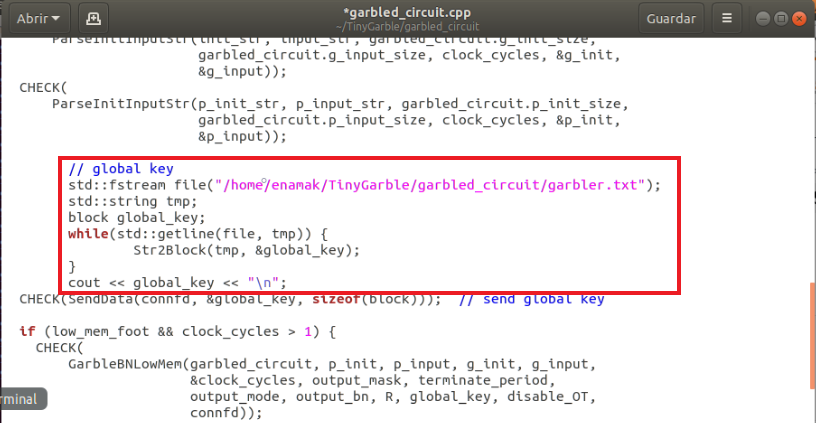
\includegraphics[width=1\textwidth, height=5.5cm]{./sdf/secure_multiparty_computation/figures/key_file.png}
    \caption{Reading Garbler's key from a file.}\label{fig:key_file}
\end{figure}

The figure above is showing a piece of the modified GarbleStr function, the same would have to be done at the EvaluatorStr function with the respective path for the evaluator keys. The absolute(starting from the root) path has to be given. "\#Include <fstream>" is also needed at the top of the file.

To apply any changes made to the file, go to TinyGarble/bin and run the "make" command.

\subsubsection{Moda function}

Since the input of the function both for Alice and Bob is a series of numbers, and since TinyGarble's iinput is in hexadecimal, we can read each digit as bcd, and easily get the total by multiplying the current number by 10 and summing the digit. Instead of using a ',' any value beetween a and f can be used.

The following fucntion was wriitten in VHDL:

\begin{lstlisting}[caption={moda.vhd}, language=Verilog, captionpos=b]

module moda(clk,  rst, g_input, e_input, o);

  input clk,  rst;
  input [1023:0] g_input, e_input; // Up to 256 hexa chars, sent from the testbench
  output [8:0] o; // With 256 hexa chars the max of different numbers is 512 (256 / 2 (commas) * 4)

  wire clk,  rst;
  reg [8:0] o;

  reg [9:0] g_iterator, e_iterator; // Represent up to the number 1023, to iterate the inputs
  wire [3:0] g_tmp, e_tmp; // To hold the current hexa char beeing checked
  reg [29:0] g_number, e_number; // Maximum of around 1 trillion, (10 hexa digits, because in bcd)
  reg g_end, e_end, g_start, e_start, g_blocked, e_blocked; // Control registers

  reg [30:0] bigger; // Hold the bigger number, one bit bigger than the biggest number for the inputs
  reg [8:0] biggerKey, counter; // Same as output

  reg [2:0] State;

  // Wires, constantly receiving the current value of their corresponding input with the current interator
  assign g_tmp = g_input[g_iterator -: 4]; // -: notacao SystemVerilog, ver se funcioa com yosys
  assign e_tmp = e_input[e_iterator -: 4];


always @(posedge clk) begin

	
    if ( rst) begin
      State <= 0;
      o = 0;
    end else begin

	    case(State)
	    0 : begin

		g_iterator <= 1023;
		e_iterator <= 1023;
		g_number <= 0;
		e_number <= 0;
		g_blocked <= 0;
		e_blocked <= 0;

		g_end <= 0;
		e_end <= 0;

		bigger <= 0;
		biggerKey <= 0;
		counter <= 0;

		State <= 1;

	    end
	    1 : begin
	      // Se ainda nao tiver chegado ao ultimo digito it ao proximo
	      if(g_blocked == 0) begin
		if(g_iterator < 4)
		  g_end <= 1;
		else
		  g_iterator <= g_iterator - 4;
	      end
	      if(e_blocked == 0) begin
		if(e_iterator < 4)
		  e_end <= 1;
		else begin
		  e_iterator <= e_iterator - 4;
		end
	      end
	      State <= 2;
	    end
	    2 : begin
	      if(g_blocked == 1 & e_blocked == 1)
		State <= 3;
	      else begin
		if(g_tmp == 10 | g_end == 1)
		  g_blocked <= 1;
		else
		  g_number <= (g_number * 10) + g_tmp;
		if(e_tmp == 10 | e_end == 1)
		  e_blocked <= 1;
		else
		  e_number <= (e_number * 10) + e_tmp;
		State <= 1;
	      end;
	    end
	    3 : begin
	      if(g_number + e_number > bigger) begin
		$display("Found bigger");
		bigger <= g_number + e_number;
		biggerKey <= counter;
	      end
	      counter <= counter + 1;
	      g_number <= 0;
	      g_blocked <= 0;
	      e_number <= 0;
	      e_blocked <= 0;
	      if(g_end == 1 & e_end == 1) begin
		State <= 4;
	      end else
		State <= 1;
	    end
	    4 : begin
	      o <= biggerKey + 1;
	      State <= 4;
	    end
	    default : begin
	      State <= 0;
	    end
	    endcase
	end			
  end

endmodule

\end{lstlisting}

When running a testbench of the above with the g\_input = 80'h421a425a9a23a412a432, and e\_input = 80'h94a420a83a902a74a821,  the result is the below:

\begin{figure}[H]
	\centering
	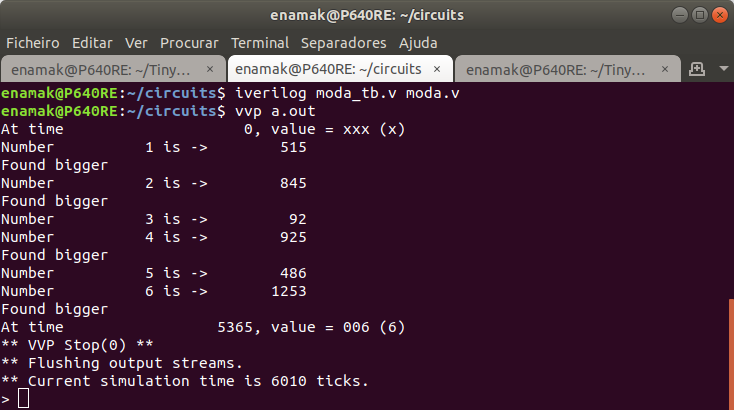
\includegraphics[width=1\textwidth, height=7cm]{./sdf/secure_multiparty_computation/figures/moda_execution_testbench.png}
    \caption{Moda's testbench execution}\label{fig:moda_execution}
\end{figure}

Converting the file to Netlist Verilog wasnt a problem besides having to delete all those weird lines mentioned above.
When trying to converto to Scd it gives the error:

\begin{figure}[H]
	\centering
	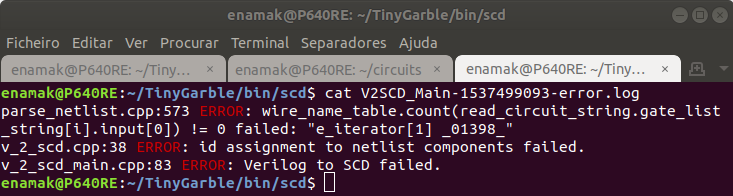
\includegraphics[width=1\textwidth, height=4cm]{./sdf/secure_multiparty_computation/figures/tinygarble_moda_scd_fail.png}
    \caption{Model SCD conversion fail}\label{fig:moda_scd_fail}
\end{figure}


% bibliographic references for the section ----------------------------
\clearpage
\printbibliography[heading=subbibliography]
\end{refsection}
\addcontentsline{toc}{subsection}{Bibliography}
\cleardoublepage
% --------------------------------------------------------------------
